\documentclass[11pt,a4paper]{article}

% Pacotes essenciais
\usepackage[utf8]{inputenc}
\usepackage[T1]{fontenc}
\usepackage{lmodern}
\usepackage[portuguese]{babel}
\usepackage{graphicx}
\usepackage{amsmath}
\usepackage{amsfonts}
\usepackage{amssymb}
\usepackage{float}
\usepackage{caption}
\usepackage{subcaption}
\usepackage{xcolor}
\usepackage{colortbl}
\usepackage{fancyhdr}
\usepackage{geometry}
\usepackage{titlesec}
\usepackage{lipsum}
\usepackage[round,authoryear]{natbib}
\usepackage{booktabs}
\usepackage{array}
\usepackage{enumitem}
\usepackage{tikz}
\usetikzlibrary{shapes.geometric}
\usepackage[hidelinks]{hyperref}

% Definição das cores
\definecolor{headercolor}{HTML}{b11116}
\definecolor{secondarycolor}{HTML}{3a5461}

% Configuração da página
\geometry{
    a4paper,
    top=2.8cm,
    bottom=2.5cm,
    left=2.5cm,
    right=2.5cm,
    headheight=1.2cm,
    headsep=0.5cm
}

% Configuração do cabeçalho
\pagestyle{fancy}
\fancyhf{}
\renewcommand{\headrulewidth}{0pt}
\renewcommand{\footrulewidth}{0.5pt}

\fancyhead[L]{%
    \begin{tikzpicture}[remember picture, overlay]
        \fill[headercolor] (current page.north west) rectangle ([yshift=-1.2cm]current page.north east);
        \node[anchor=west, inner sep=0pt] at ([xshift=1cm, yshift=-0.6cm]current page.north west) 
            {
\includegraphics[height=0.8cm]{imgs/base/fatec-rgt.png}};
        \node[anchor=east, inner sep=0pt] at ([xshift=-1cm, yshift=-0.6cm]current page.north east) 
            {
\includegraphics[height=0.9cm]{imgs/base/cps-logo.png}};
        \node[anchor=east, inner sep=0pt] at ([xshift=-2.8cm, yshift=-0.6cm]current page.north east) 
            {
\includegraphics[height=1.05cm]{imgs/base/governo-sp-secretaria-logo.png}};
    \end{tikzpicture}
}

\fancyfoot[L]{\footnotesize\textcolor{secondarycolor}{Faculdade de Tecnologia do Estado de São Paulo\\ fatecregistro.cps.sp.gov.br}}
\fancyfoot[R]{\thepage}

% Configuração dos títulos das seções
\titleformat{\section}
    {\normalfont\large\bfseries\color{secondarycolor}}
    {\thesection}{1em}{}

\titleformat{\subsection}
    {\normalfont\normalsize\bfseries\color{secondarycolor}}
    {\thesubsection}{1em}{}

\begin{document}

% ===== CAPA =====
\begin{titlepage}
    \centering
    
    % Logos no topo
    \begin{tikzpicture}[remember picture, overlay]
        \fill[headercolor] (current page.north west) rectangle ([yshift=-1.2cm]current page.north east);
        \node[anchor=west, inner sep=0pt] at ([xshift=1cm, yshift=-0.6cm]current page.north west) 
            {
\includegraphics[height=0.8cm]{imgs/base/fatec-rgt.png}};
        \node[anchor=east, inner sep=0pt] at ([xshift=-1cm, yshift=-0.6cm]current page.north east) 
            {
\includegraphics[height=0.9cm]{imgs/base/cps-logo.png}};
        \node[anchor=east, inner sep=0pt] at ([xshift=-2.8cm, yshift=-0.6cm]current page.north east) 
            {
\includegraphics[height=1.05cm]{imgs/base/governo-sp-secretaria-logo.png}};
    \end{tikzpicture}
    
    \vspace*{3.5cm}
    
    % Nome da faculdade
    {\normalsize FACULDADE DE TECNOLOGIA DO ESTADO DE SÃO PAULO\par}
    \vspace{0.5cm}
    
    % Curso
    {\normalsize DESENVOLVIMENTO DE SOFTWARE MULTIPLATAFORMA\par}
    
    \vspace{4cm}
    
    % Artefatos do Projeto de Software
    {\normalsize ARTEFATOS DO PROJETO DE SOFTWARE\par}
    
    \vspace{0.3cm}
    
    % Nome do projeto
    {\normalsize Teste de Desempenho Contínuo, Orientado por Rastreamento Ocular\par}
    
    \vspace{3cm}
    
    % Autores
    {\normalsize
    Amanda de Oliveira Costa\\
    Arthur Ribeiro Dias Fudali\\
    Diego Baltazar de Souza Claudio\\
    Giovana da Silva Albanês Santos\\
    Igor Leite Gomes
    }
    
    \vfill
    
    % Rodapé
    {\small Registro -- SP\\
    2026}
    
\end{titlepage}

% Força o cabeçalho em todas as páginas
\pagestyle{fancy}

% ===== SUMÁRIO =====
\tableofcontents
\newpage

% ===== CANVAS =====
\section{CANVAS: Modelo de Negócio e Estratégia}

O Business Model Canvas \cite{santos2024} é uma ferramenta visual estratégica\footnote{O Canvas foi desenvolvido por Alexander Osterwalder e é amplamente utilizado em startups e empresas estabelecidas para modelagem de negócios.} que permite descrever, analisar e projetar modelos de negócio de forma clara e objetiva. O canvas é dividido em nove blocos fundamentais que cobrem as principais áreas de um negócio.

Esse modelo de negócios foi estruturado de acordo com os nove blocos do Canvas, permitindo visualizar de forma integrada os principais elementos que compõem a proposta de valor, os recursos, os canais e a estrutura operacional do projeto FocusQuest.

Os Segmentos de Clientes alvo compreendem clínicas de neuropsicologia e psiquiatria, profissionais autônomos da saúde mental e instituições de reabilitação cognitiva. A Proposta de Valor consiste em desenvolver um serious game que avalia a atenção sustentada, impulsividade e tempo de resposta com base no Teste de Desempenho Contínuo (TDC), devolvendo um feedback imediato do resultado para cada usuário.

Os Canais de entrega envolvem o uso de computadores com câmeras e acesso à internet, com o sistema devidamente hospedado em servidor. O Relacionamento com o Cliente baseia-se em testes gamificados e interativos que permitem a geração de um pré-diagnóstico rápido por meio de um layout simples e intuitivo.

As Fontes de Renda são viabilizadas através de anúncios na internet, do tráfego no website, da disponibilidade do software para download e do sistema de recomendações de outros usuários. Entre os Recursos-Chave, destacam-se a facilidade de uso do software, a alta interatividade e a conveniência de gerar relatórios automatizados com interpretação de resultados.

As Atividades-Chave compreendem a criação de conteúdo educacional, o desenvolvimento e manutenção do sistema, além do suporte contínuo ao usuário. Os Parceiros-Chave foram identificados como as próprias clínicas de saúde mental e o usuário final, que colaboram com o ecossistema do projeto.

Por fim, a Estrutura de Custos é dividida entre custos fixos, como internet, hospedagem e investimento em tráfego pago, e custos variáveis, que abrangem o desenvolvimento de software, marketing, suporte e o patrocínio de especialistas em neuropsicologia e psiquiatria para validação do sistema.

\begin{table}[H]
\centering
\caption{Business Model Canvas -- PI - FocusQuest}
\label{tab:canvas}
\small
\begin{tabular}{|p{2.6cm}|p{2.6cm}|p{3.2cm}|p{2.6cm}|p{2.8cm}|}
\hline
\textbf{1. Segmento de clientes} & \textbf{2. Proposta de valor} & \textbf{3. Canais} & \textbf{4. Relacionamento} & \textbf{5. Fontes de renda} \\
\hline
Clínicas de neuropsicologia e psiquiatria \newline Profissionais da saúde mental autônomos \newline Instituições de reabilitação cognitiva
&
Desenvolver um serious game que avalia atenção sustentada, impulsividade e tempo de resposta com base no Teste de Desempenho Contínuo (TDC) \newline Devolver um Feedback do resultado do teste de cada usuário
&
Computador com camera e acesso a internet \newline Hospedagem em servidor
&
Testes Gameficados e Interativos \newline Geração de um Pré-diagnóstico rápido \newline Layout Simples e Intuitivo
&
Anuncios na internet \newline Website \newline Disponibilidade para Download \newline Recomendações de outros usuários \\
\hline
& \textbf{6. Recursos chave} & & \textbf{7. Atividades chave} & \\
\hline
& Software de uso fácil \newline Teste Gameficado e Interativo \newline Feedback gamificado para o usuário final \newline Conveniencia de ter um pré-diagnóstico \newline Alta interatividade \newline Relatórios automatizados com interpretação de resultados
& &
Criação de conteúdo educacional \newline Desenvolvimento de software \newline Manutenção do sistema \newline Suporte ao usuário &
\\
\hline
\multicolumn{2}{|p{5.5cm}|}{\textbf{8. Parceiros chave}} & \multicolumn{3}{p{9.4cm}|}{\textbf{9. Estrutura de custos}} \\
\hline
\multicolumn{2}{|p{5.5cm}|}{Clínicas de saúde mental \newline Usuário final} & \multicolumn{3}{p{9.4cm}|}{Custos fixos: internet, hospedagem do programa, infraestrutura, investimento em tráfego pago \newline Custos variáveis: Desenvolvimento de software, manutenção de software, custo de marketing e divulgação, patrocínio de especialistas em neuropsicologia e psiquiatria, custo de testes com usuários, custo de recrutamento e formação de usuários, custo de suporte ao usuário} \\
\hline
\end{tabular}
\end{table}

Esse artefato auxilia na visualização estratégica do projeto FocusQuest, evidenciando sua
viabilidade técnica e comercial, além de integrar as dimensões tecnológicas, clínicas e de mercado do
produto proposto.

% ===== SWOT =====
\section{SWOT: Análise Estratégica}

A Análise SWOT (Strengths, Weaknesses, Opportunities, Threats) ou FOFA (Forças, Oportunidades, Fraquezas e Ameaças) \cite{oliveira2023} é uma ferramenta fundamental para planejamento estratégico\footnote{A análise SWOT foi criada na década de 1960 por Albert Humphrey no Stanford Research Institute.} que permite identificar fatores internos e externos que impactam o projeto. Analisa forças, fraquezas, oportunidades e ameaças do projeto.

\subsubsection{Fatores Internos: O Core do Projeto}

No âmbito interno, o projeto destaca-se pela \textbf{Inovação Biométrica}. O uso de \textit{eye-tracking} em um ambiente gamificado transforma uma tarefa clínica geralmente exaustiva em uma experiência de alto engajamento, o que aumenta a fidelidade dos dados coletados e reduz a taxa de abandono do teste. 

Por outro lado, a \textbf{Dependência de Hardware} é um ponto de atenção crítico. A eficácia da ferramenta está atrelada à qualidade da câmera e às condições de iluminação do usuário final. Isso exige um esforço contínuo em otimização de software e algoritmos de calibração para garantir que a solução seja acessível e confiável em diversos cenários domésticos ou clínicos.

\subsubsection{Fatores Externos: Oportunidades e Resiliência}

O cenário externo revela um terreno fértil para a \textbf{Expansão Digital} na saúde. A crescente aceitação da telemedicina e da triagem remota abre portas para parcerias B2B (\textit{Business-to-Business}) com clínicas e instituições de ensino, posicionando o \textit{FocusQuest} como uma solução de baixo custo e alta escalabilidade. 

Entretanto, o projeto opera em um setor altamente regulado. A conformidade com a \textbf{LGPD (Lei Geral de Proteção de Dados)} e as normas de saúde representam ameaças estruturais que exigem rigor técnico e jurídico. Além disso, a possível entrada de grandes \textit{players} de \textit{MedTech} exige que o projeto mantenha agilidade na inovação e foco na experiência do usuário para preservar sua diferenciação de mercado.

\subsubsection{Síntese e Direcionamento}

Em suma, a SWOT indica que o sucesso do \textit{FocusQuest} depende da capacidade de converter sua superioridade técnica e científica em uma ferramenta de fácil adoção. O foco estratégico imediato reside em reduzir as barreiras técnicas de entrada enquanto se fortalecem as barreiras de saída através do rigor científico e da fidelização dos profissionais da área.

\begin{table}[H]
\centering
\caption{Análise SWOT Estratégica - Projeto FocusQuest}
\label{tab:swot}
\small
\begin{tabular}{|p{7.2cm}|p{7.2cm}|}
\hline
\multicolumn{2}{|c|}{\cellcolor{gray!20}\textbf{FATORES INTERNOS (Contornáveis)}} \\
\hline
\textbf{FORÇAS (Strengths)} & \textbf{FRAQUEZAS (Weaknesses)} \\
\hline
\begin{minipage}[t]{7cm}
\begin{itemize}[leftmargin=*]
    \item \textbf{Inovação Biométrica:} Diferencial competitivo com uso de \textit{eye-tracking} acessível.
    \item \textbf{Engajamento:} Metodologia de \textit{Serious Game} que reduz o abandono em testes clínicos.
    \item \textbf{Rigor Científico:} Alinhamento técnico com o protocolo TDC (Teste de Desempenho Contínuo).
\end{itemize}
\end{minipage}
&
\begin{minipage}[t]{7cm}
\begin{itemize}[leftmargin=*]
    \item \textbf{Dependência de Hardware:} Sensibilidade a variações de iluminação e qualidade de câmeras externas.
    \item \textbf{Barreiras de Dados:} Complexidade na aquisição de bases de dados clínicas robustas para validação.
    \item \textbf{Calibração:} Necessidade de ajuste inicial que pode afetar a experiência do usuário.
\end{itemize}
\end{minipage}
\\
\hline
\multicolumn{2}{|c|}{\cellcolor{gray!20}\textbf{FATORES EXTERNOS (Incontroláveis)}} \\
\hline
\textbf{OPORTUNIDADES (Opportunities)} & \textbf{AMEAÇAS (Threats)} \\
\hline
\begin{minipage}[t]{7cm}
\begin{itemize}[leftmargin=*]
    \item \textbf{Expansão Digital:} Crescente demanda por ferramentas de triagem remota e telemedicina.
    \item \textbf{Parcerias B2B:} Potencial de adoção por instituições de ensino e clínicas neuropsicológicas.
    \item \textbf{Diferenciação de Mercado:} Inexistência de soluções gamificadas semelhantes no cenário nacional.
\end{itemize}
\end{minipage}
&
\begin{minipage}[t]{7cm}
\begin{itemize}[leftmargin=*]
    \item \textbf{Compliance e LGPD:} Rigor na proteção de dados sensíveis e diagnósticos de saúde.
    \item \textbf{Barreiras de Adoção:} Resistência de profissionais tradicionais a métodos de triagem automatizados.
    \item \textbf{Concorrência:} Entrada de grandes \textit{players} de MedTech com maior capacidade de investimento.
\end{itemize}
\end{minipage}
\\
\hline
\end{tabular}
\end{table}


\subsection{Recomendações Estratégicas}

Com base no cruzamento das variáveis da análise SWOT, as diretrizes estratégicas para o desenvolvimento do \textit{FocusQuest} devem focar em quatro eixos de atuação:

\begin{itemize}
    \item \textbf{Estratégias Ofensivas (Forças + Oportunidades):} Explorar a \textbf{Inovação Biométrica} (eye-tracking) para posicionar o produto como líder no nicho de triagem remota e telemedicina, utilizando a gamificação como diferencial de mercado frente a métodos tradicionais.
    
    \item \textbf{Estratégias de Confronto (Forças + Ameaças):} Utilizar o \textbf{Rigor Científico} (alinhamento ao TDC) e os dados de engajamento para mitigar a resistência de profissionais tradicionais, estabelecendo o sistema como uma ferramenta de apoio diagnóstico confiável e difícil de ser replicada por concorrentes genéricos.
    
    \item \textbf{Estratégias de Reforço (Fraquezas + Oportunidades):} Firmar parcerias estratégicas \textbf{B2B} com clínicas e instituições de ensino para facilitar a coleta de bases de dados clínicas, superando a barreira de validação e acelerando o aprimoramento dos algoritmos de rastreamento.
    
    \item \textbf{Estratégias Defensivas (Fraquezas + Ameaças):} Estabelecer protocolos rígidos de \textbf{Compliance e LGPD} para proteção de dados sensíveis e investir em UX (\textit{User Experience}) para simplificar a calibração de hardware, evitando que limitações técnicas ou burocráticas abram espaço para a concorrência.
\end{itemize}

% ===== UX/UI =====
\section{UX/UI: Design de Interface e Experiência do Usuário}

UX (User Experience) e UI (User Interface) \cite{silva2025} são disciplinas complementares focadas em criar produtos digitais que sejam funcionais, acessíveis e agradáveis de usar. O UX concentra-se na experiência geral do usuário, enquanto o UI cuida dos elementos visuais e interativos.

\begin{figure}[H]
\centering
\begin{minipage}{0.45\textwidth}
    \centering
    \fbox{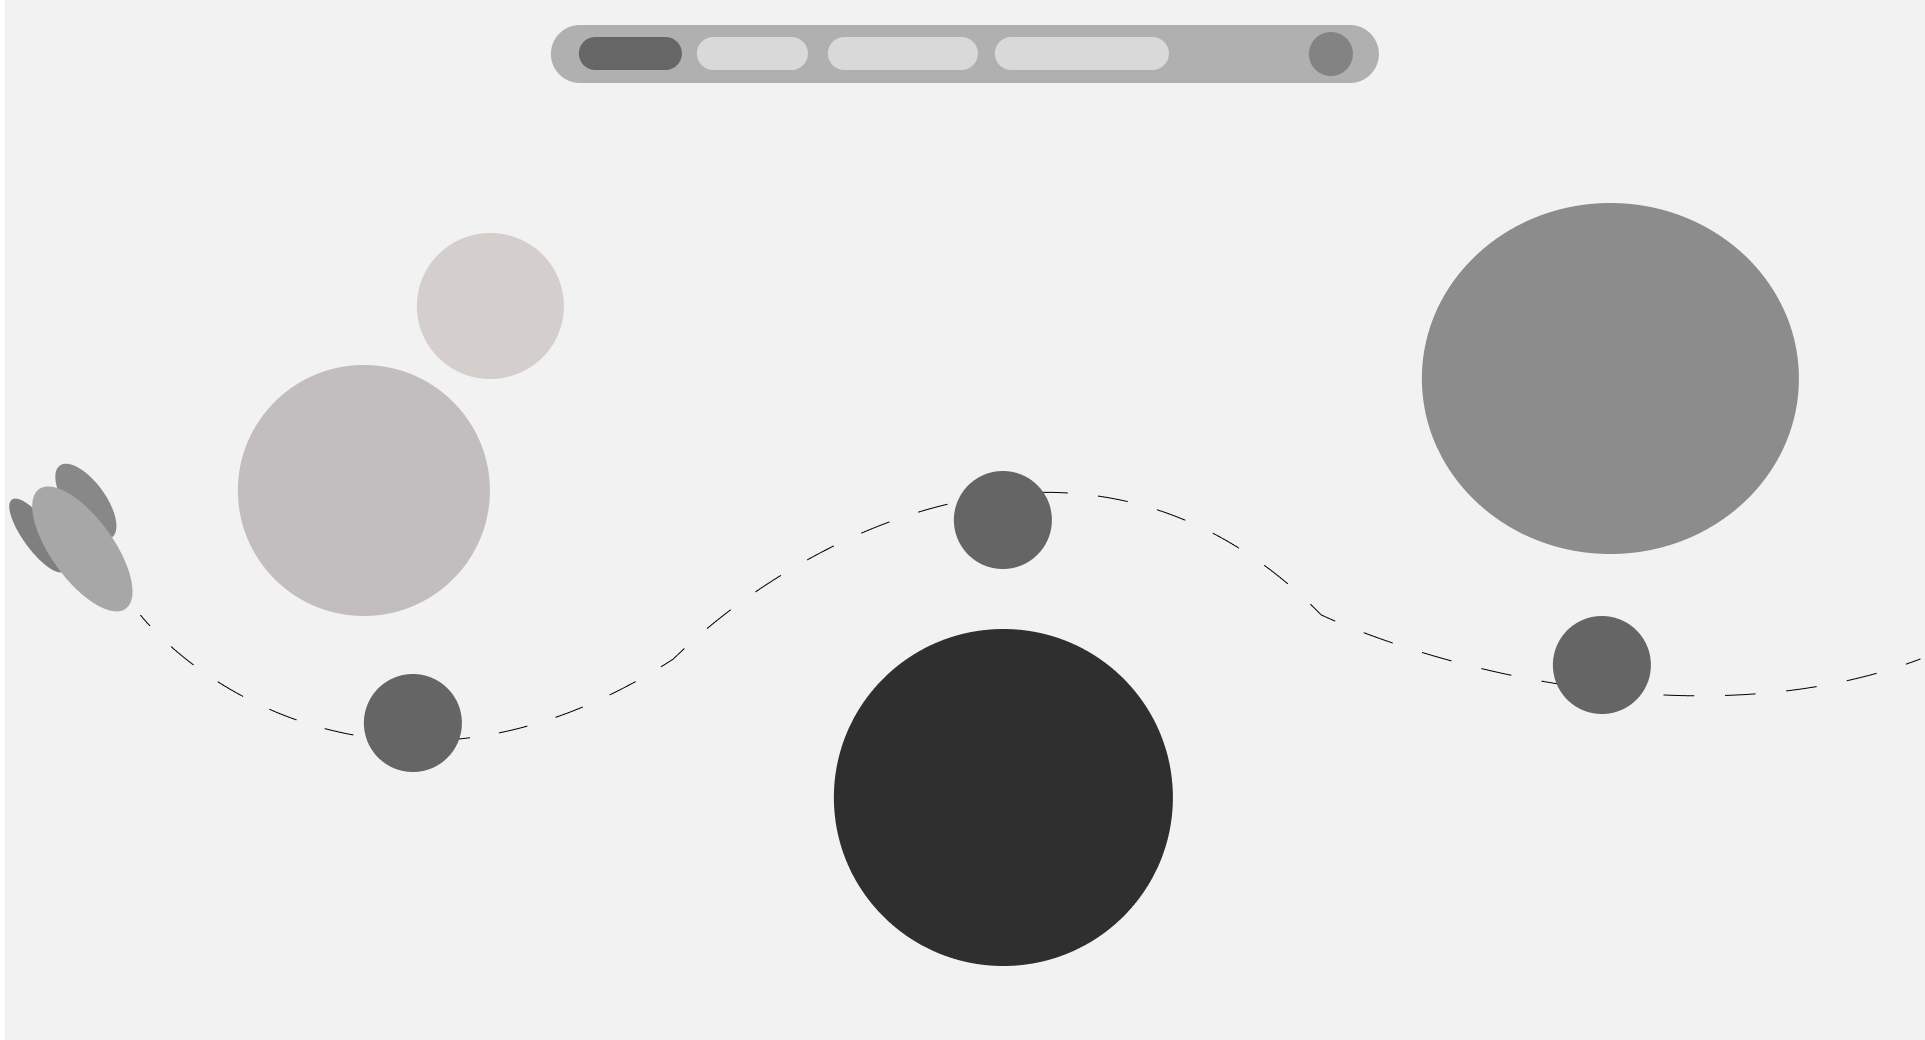
\includegraphics[width=0.9\textwidth]{imgs/wireframe.png}}
    \caption{Wireframe da tela inicial}
    \label{fig:wireframe}
\end{minipage}
\hfill
\begin{minipage}{0.45\textwidth}
    \centering
    \fbox{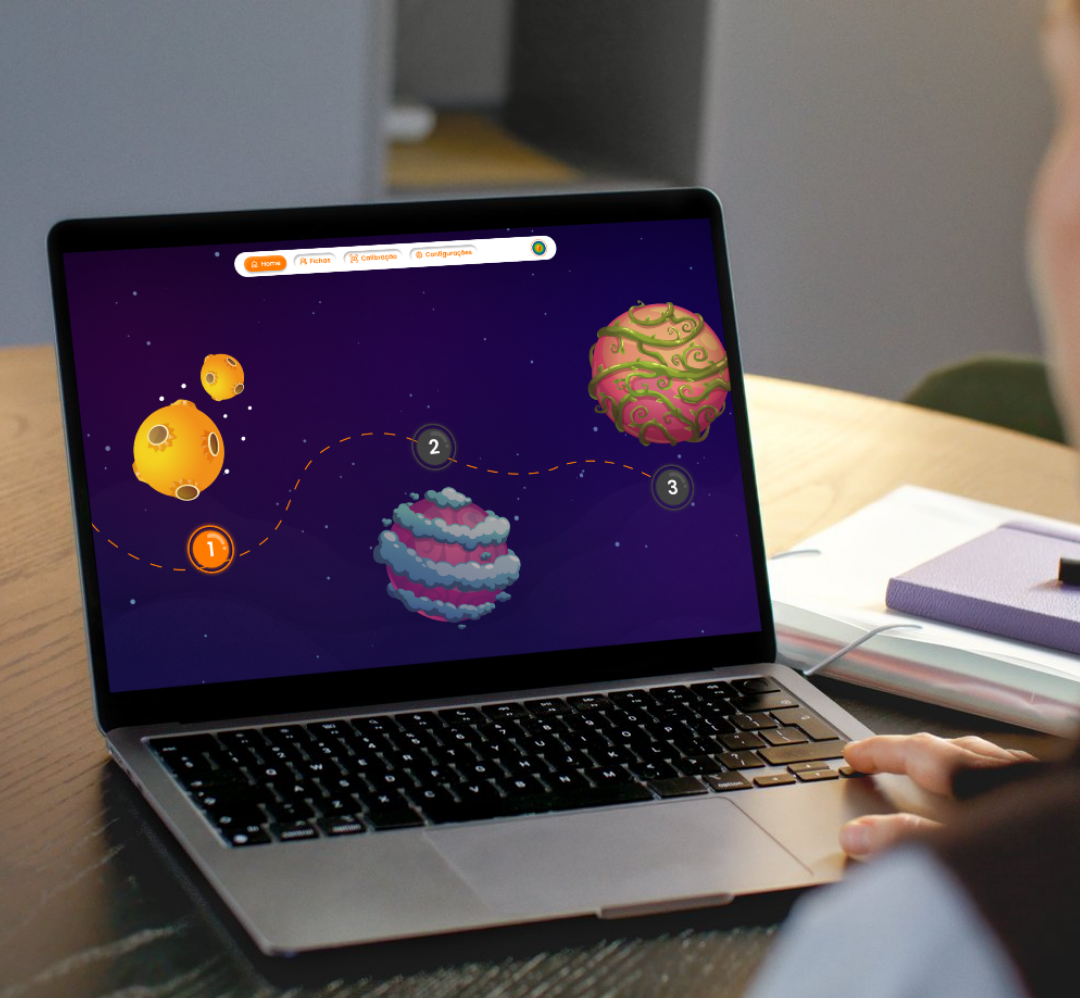
\includegraphics[width=0.9\textwidth]{imgs/mockup.png}}
    \caption{Mockup de alta fidelidade}
    \label{fig:mockup}
\end{minipage}
\end{figure}

\subsection{Protótipo}

O protótipo do projeto foi desenvolvido utilizando a ferramenta Figma, ferramenta de design poderosa e colaborativa para equipes.

\subsection{Guia de Estilos}

\begin{table}[H]
\centering
\caption{Paleta de Cores do Projeto}
\label{tab:cores}
\begin{tabular}{|l|c|l|l|}
\hline
\textbf{Elemento} & \textbf{Cor} & \textbf{Código HEX} & \textbf{Uso} \\
\hline
Primária & \colorbox[HTML]{FF7B00}{\phantom{AAA}} & \#FF7B00 & Botões principais, destaques, Títulos \\
Texto & \colorbox[HTML]{3B3B3B}{\phantom{AAA}} & \#3B3B3B & Texto principal \\
Fundo & \colorbox[HTML]{FFFFFF}{\phantom{AAA}} & \#FFFFFF & Background padrão \\
Sucesso & \colorbox[HTML]{00c950}{\phantom{AAA}} & \#00c950 & Mensagens de sucesso \\
Erro & \colorbox[HTML]{fb2c36}{\color{white}\phantom{AAA}} & \#fb2c36 & Mensagens de erro \\
\hline
\end{tabular}
\end{table}

% ===== WEBSITE =====
\section{Website: Estrutura e Especificações Técnicas Web}

\subsection{Mapa do Site da Equipe}

O mapa do site (sitemap) mostra a hierarquia e organização das páginas do website da equipe:

\begin{figure}[H]
\centering
\begin{tikzpicture}[
    level 1/.style={sibling distance=4cm, level distance=1.5cm},
    level 2/.style={sibling distance=2cm, level distance=1.5cm},
    every node/.style={rectangle, draw, rounded corners, 
                       fill=secondarycolor!20, 
                       text width=2.5cm, 
                       align=center,
                       font=\small}
]
\node {Home}
    child {node {Quem somos}
        child {node {História}}
        child {node {Missão, Visão e Valores}}
    }
    child {node {FocusQuest}}
    child {node {Equipe}}
    child {node {Contato}};
\end{tikzpicture}
\caption{Estrutura de navegação do website da equipe}
\label{fig:sitemap}
\end{figure}

\subsection{Conteúdo das Páginas}

\textbf{Páginas principais do site da equipe:}

\begin{itemize}
    \item \textbf{Home:} Apresentação da equipe e logo
    \item \textbf{Quem somos:} História da equipe, missão, visão e valores
    \item \textbf{FocusQuest:} Descrição do projeto, objetivos e mockup
    \item \textbf{Equipe:} Perfil dos membros (nome, foto, função, LinkedIn/GitHub/Instagram)
    \item \textbf{Contato:} Formulário de contato e e-mail
\end{itemize}

\subsection{Especificações Técnicas do Site da Equipe}

\begin{table}[H]
\centering
\caption{Stack Tecnológica do Website da Equipe}
\label{tab:stack-web}
\begin{tabular}{|l|l|p{6cm}|}
\hline
\textbf{Camada} & \textbf{Tecnologia} & \textbf{Descrição} \\
\hline
Frontend & JavaScript & Linguagem de programação para desenvolvimento web \\
Estilização & CSS & Linguagem de estilo para definição da aparência dos elementos HTML \\
Hospedagem & Vercel & Plataforma de deploy e hosting gratuita \\
Formulário & EmailJS & Biblioteca para envio de mensagens de contato via e-mail \\
Analytics & Google Analytics & Ferramenta de métricas e análise de visitantes \\
\hline
\end{tabular}
\end{table}

% ===== DIAGRAMAS UML =====
\section{Diagramas UML: Modelagem Visual do Sistema}

A Unified Modeling Language (UML) \cite{kumar2024} é uma linguagem de modelagem visual usada para especificar, visualizar, construir e documentar artefatos de sistemas de software.\footnote{A UML foi padronizada pela Object Management Group (OMG) em 1997.}

\subsection{Diagrama de Casos de Uso}

O diagrama de casos de uso do \textit{FocusQuest} descreve as interações entre os atores principais (\textbf{Profissional de Saúde}, \textbf{Paciente} e \textbf{Administrador}) e os componentes do sistema. O processo central consiste na "Sessão de Teste", coordenada pelo profissional, que integra a calibração ocular e as três fases de avaliação do desempenho atencional. A operação é suportada tecnicamente por \textit{WebGazer}, \textit{Socket.IO} e \textit{MongoDB}, culminando na geração automática de um relatório de desempenho para auxílio no pré-diagnóstico.

\begin{figure}[H]
\centering

\includegraphics[width=\textwidth]{imgs/caso-de-uso.png}
\caption{Diagrama de Casos de Uso do Sistema}
\label{fig:use-case-diagram}
\end{figure}

\subsection{Diagrama de Classes}

O diagrama de classes do sistema \textit{FocusQuest} detalha a arquitetura estrutural e a lógica de persistência do \textit{backend}. A solução é estruturada em torno de um componente \textbf{Server} que orquestra diferentes \textbf{Handlers} e \textbf{Services} (Fases 1, 2 e 3), responsáveis por processar as regras de negócio e a interação em tempo real.  

As entidades de dados fundamentais são o \textbf{Usuário} (especialista) e o \textbf{Paciente}, com o sistema a gerir a relação de acompanhamento e a criação de \textbf{Experimentos} específicos para cada fase do teste. Estes experimentos registam métricas detalhadas, como o histórico de rastreio ocular e tempos de resposta, que são posteriormente processados pelas classes de \textbf{Estatísticas} para gerar resumos analíticos. A infraestrutura é completada por módulos de \textbf{DatabaseConnections} para persistência em MongoDB e Redis, e uma integração com \textbf{Arduino} para comunicação com dispositivos de \textit{hardware} externos.

\begin{figure}[H]
\centering

\includegraphics[width=\textwidth]{imgs/diagrama-de-classe.png}
\caption{Diagrama de Classes do Sistema}
\label{fig:class-diagram}
\end{figure}

\subsection{Diagrama de Objetos}

O diagrama de objetos apresenta um retrato do sistema \textit{FocusQuest} em tempo de execução durante uma sessão clínica, validando o fluxo de dados e a arquitetura na prática. A representação ilustra as instâncias de infraestrutura ativas (servidor e banco de dados) interligadas aos atores do processo, onde a especialista (usuário) gerencia a avaliação de um paciente. Ao longo da sessão, o sistema instancia as três fases do experimento — Foco Visual, Atenção Sustentada e Resposta a Estímulos —, registrando dados brutos como coordenadas de rastreamento ocular e interações. Em seguida, esses registros são processados automaticamente em instâncias de Estatísticas, que consolidam métricas precisas, como tempo médio de reação e total de acertos, retornando um relatório analítico pronto para a visualização da profissional e auxiliando diretamente no pré-diagnóstico.

\begin{figure}[H]
\centering
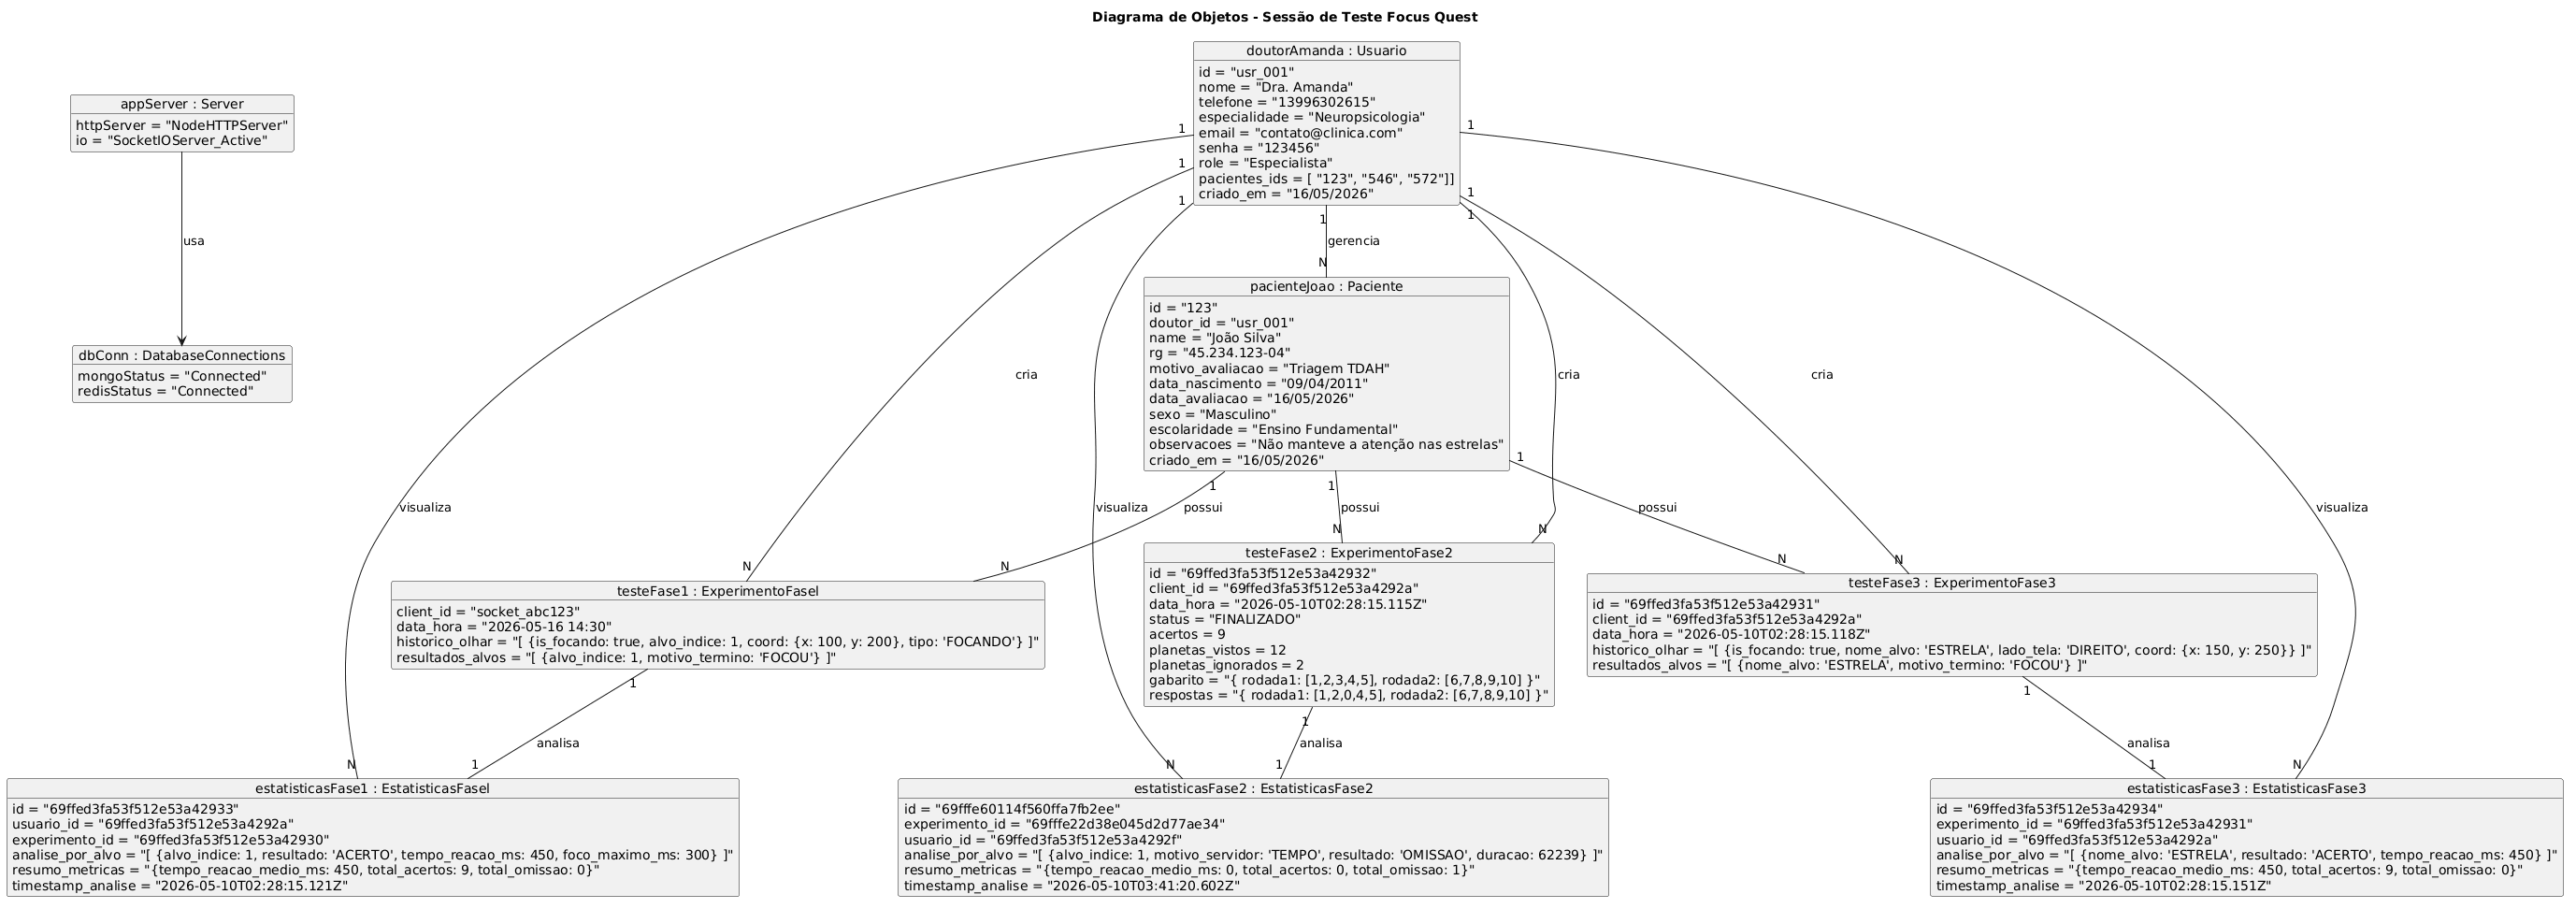
\includegraphics[width=\textwidth]{imgs/diagrama-objetos.png}
\caption{Diagrama de Objetos do Sistema}
\label{fig:object-diagram}
\end{figure}

\section{Banco de dados: Modelagem e Estruturação de Dados}

O modelo de dados do MongoDB para o \textit{FocusQuest} adota uma abordagem NoSQL orientada a documentos, otimizada para o armazenamento de dados biométricos e clínicos com alta flexibilidade. O esquema organiza-se em coleções fundamentais: \textbf{Usuários}, que gere o acesso e perfil dos profissionais de saúde; \textbf{Pacientes}, que centraliza o histórico e prontuário dos avaliados; e as coleções de \textbf{Experimentos} e \textbf{Estatísticas}, responsáveis pela persistência detalhada de cada fase do teste. A modelagem utiliza o conceito de referenciamento para manter a integridade entre especialistas e seus respectivos pacientes, permitindo que o sistema processe e recupere padrões complexos de rastreamento ocular e tempos de reação de forma eficiente para a composição dos relatórios finais.

\begin{figure}[H]
\centering
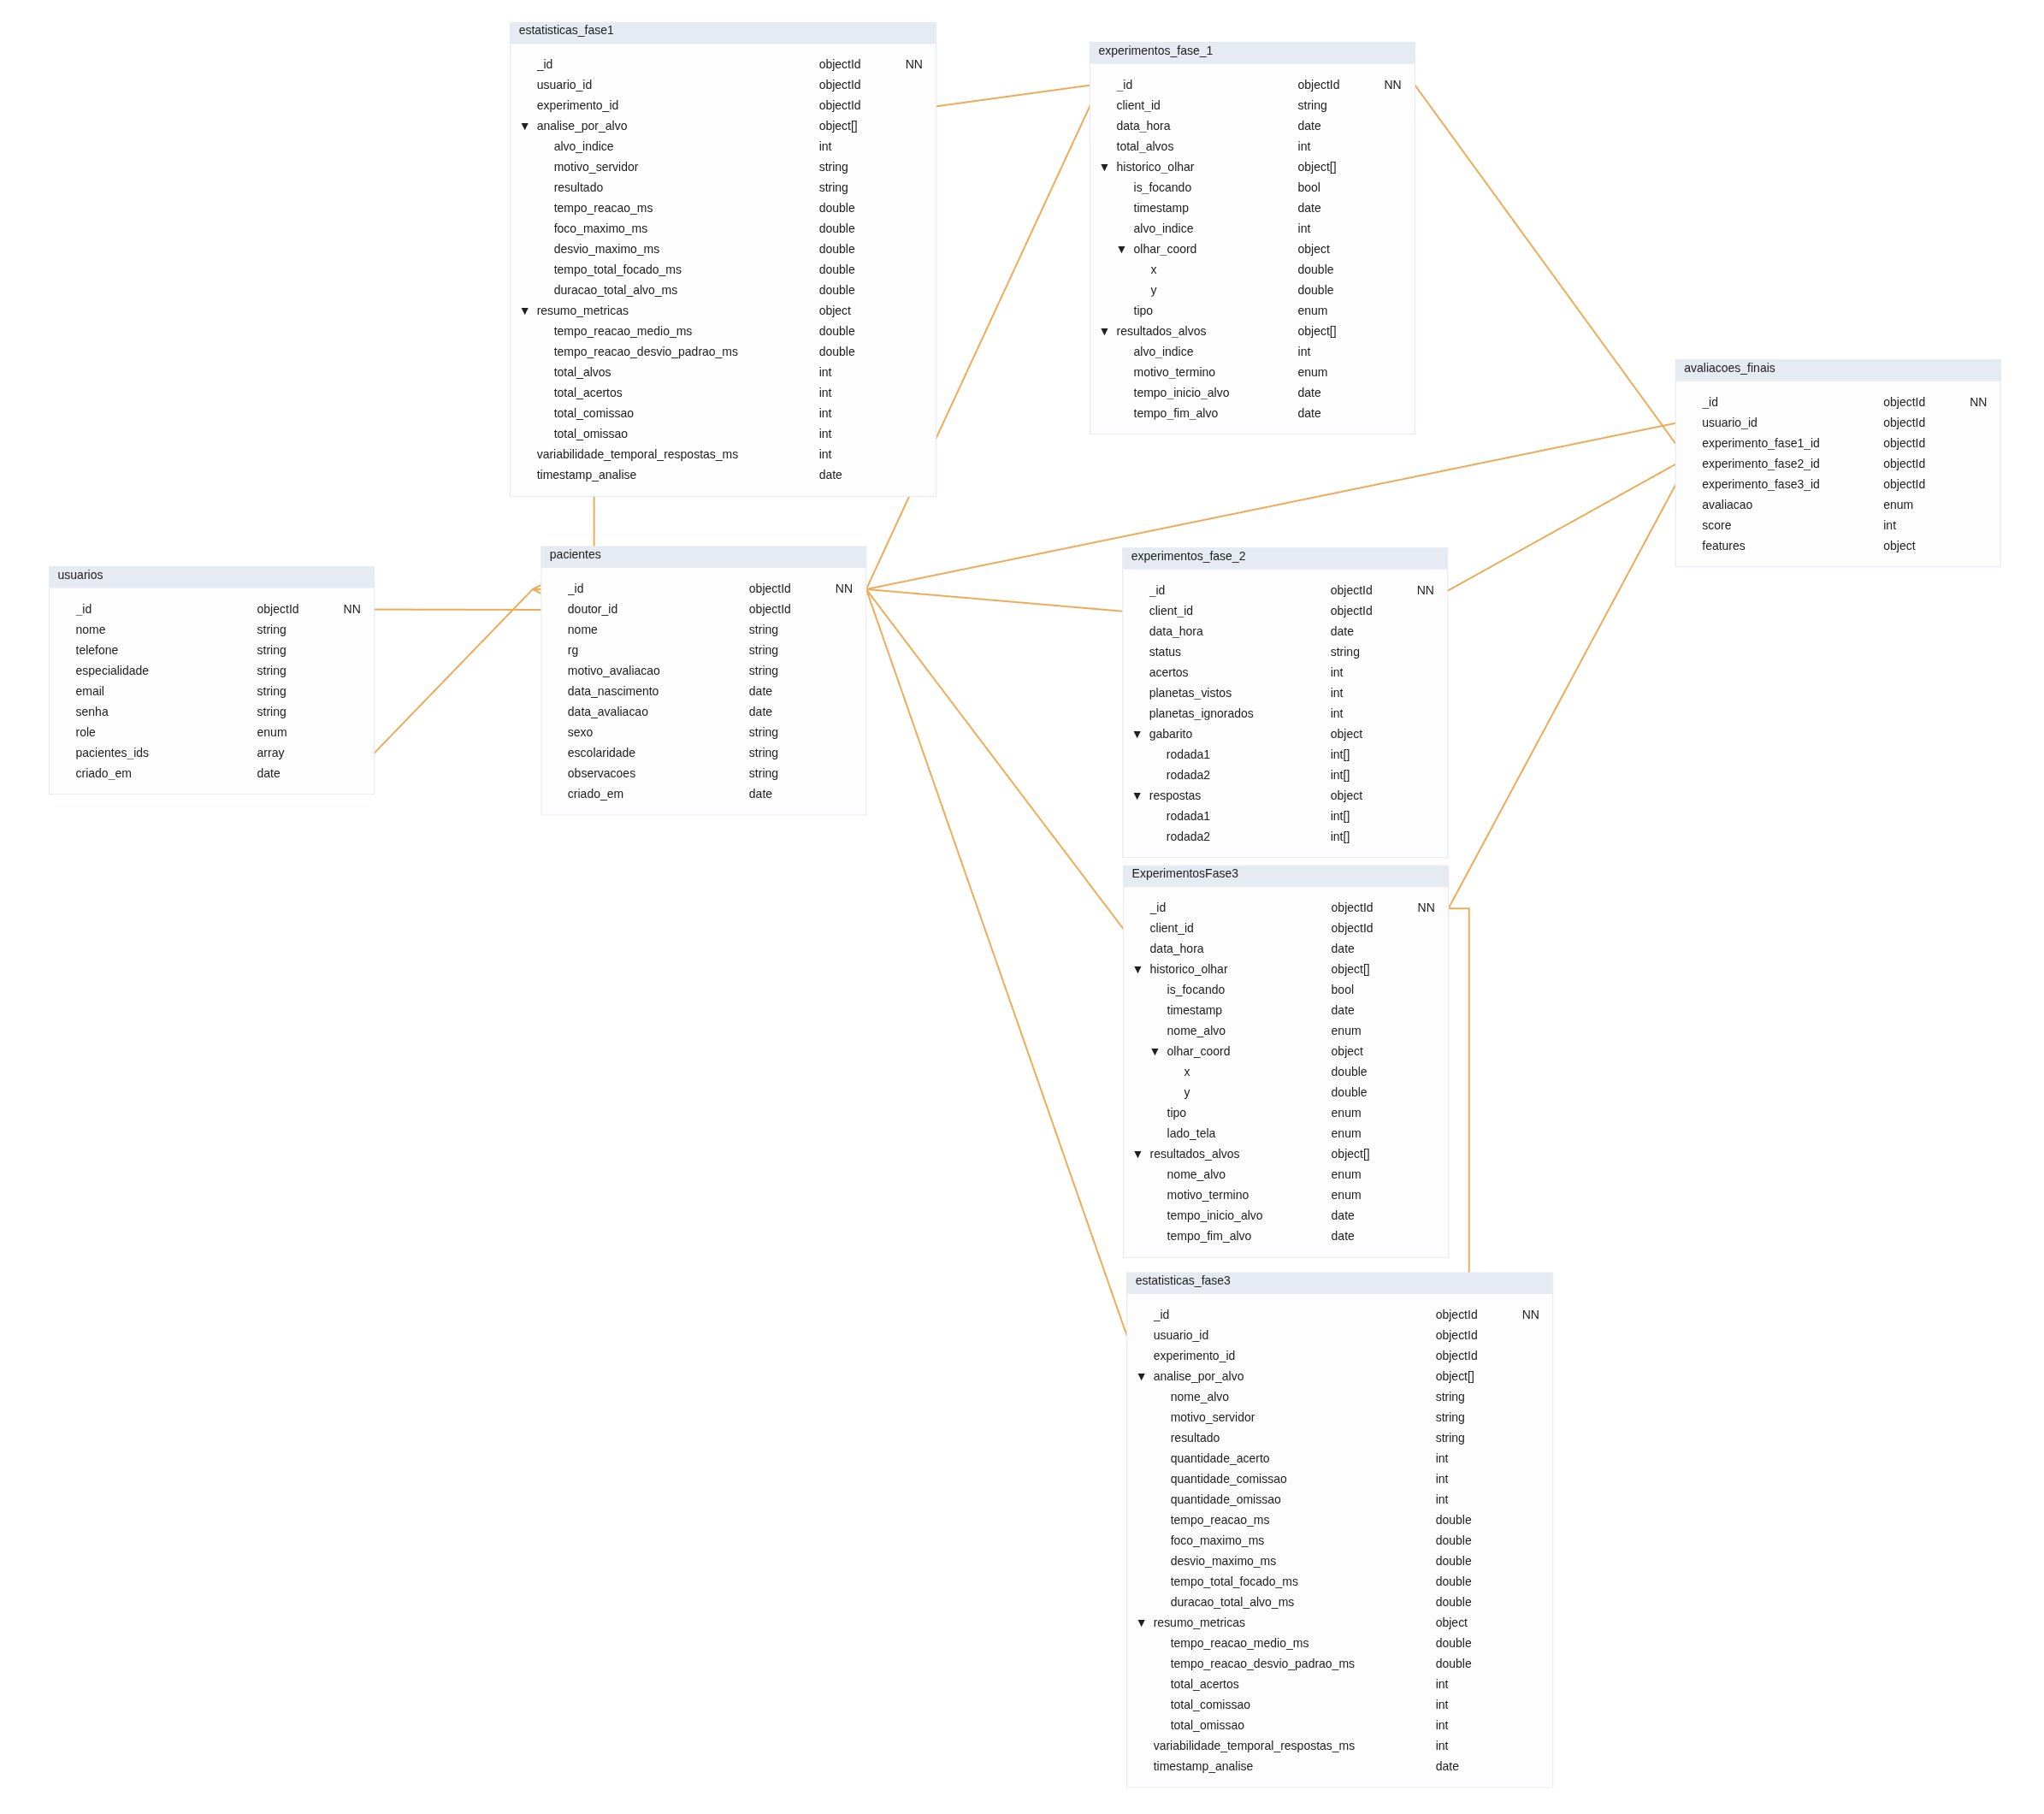
\includegraphics[width=\textwidth]{imgs/diagrama-banco.png}
\caption{Diagrama de Banco de Dados do Sistema}
\label{fig:database-diagram}
\end{figure}

% ===== DEVOPS =====

\section{DevOps: Infraestrutura, Automação e Entrega Contínua}

DevOps \cite{wang2023} é uma cultura e conjunto de práticas que integra desenvolvimento de software (Dev) e operações de TI (Ops), focando em automação, colaboração e entrega contínua.

\subsection{Diagrama de Redes}

O diagrama de redes ilustra a arquitetura de infraestrutura e o fluxo de comunicação do sistema \textit{FocusQuest}, projetado para suportar o Teste de Desempenho Contínuo orientado por visão computacional. O fluxo tem início no PC do usuário, onde ocorre a captura local dos dados de rastreamento ocular (\textit{eye-tracking}), que são transmitidos de forma segura através do roteador e do provedor de acesso à internet (ISP). Ao ingressar no ambiente de \textit{Virtual Private Cloud} (VPC), o tráfego é gerenciado e distribuído por um \textit{Cloud Load Balancing}, garantindo estabilidade antes de atingir a API responsável pela coleta de dados. Para assegurar alto desempenho e confiabilidade, a arquitetura de armazenamento combina o \textit{Memorystore} (Redis) para operações de cache em tempo real com um banco de dados \textit{Cloud NoSQL} (MongoDB) para a persistência definitiva. Complementando o ecossistema, os registros consolidados são enviados para um módulo de Inteligência Artificial de aprendizagem guiada, responsável por processar os dados biométricos e gerar os resultados preditivos sobre a atenção e o foco do paciente.

\begin{figure}[H]
\centering
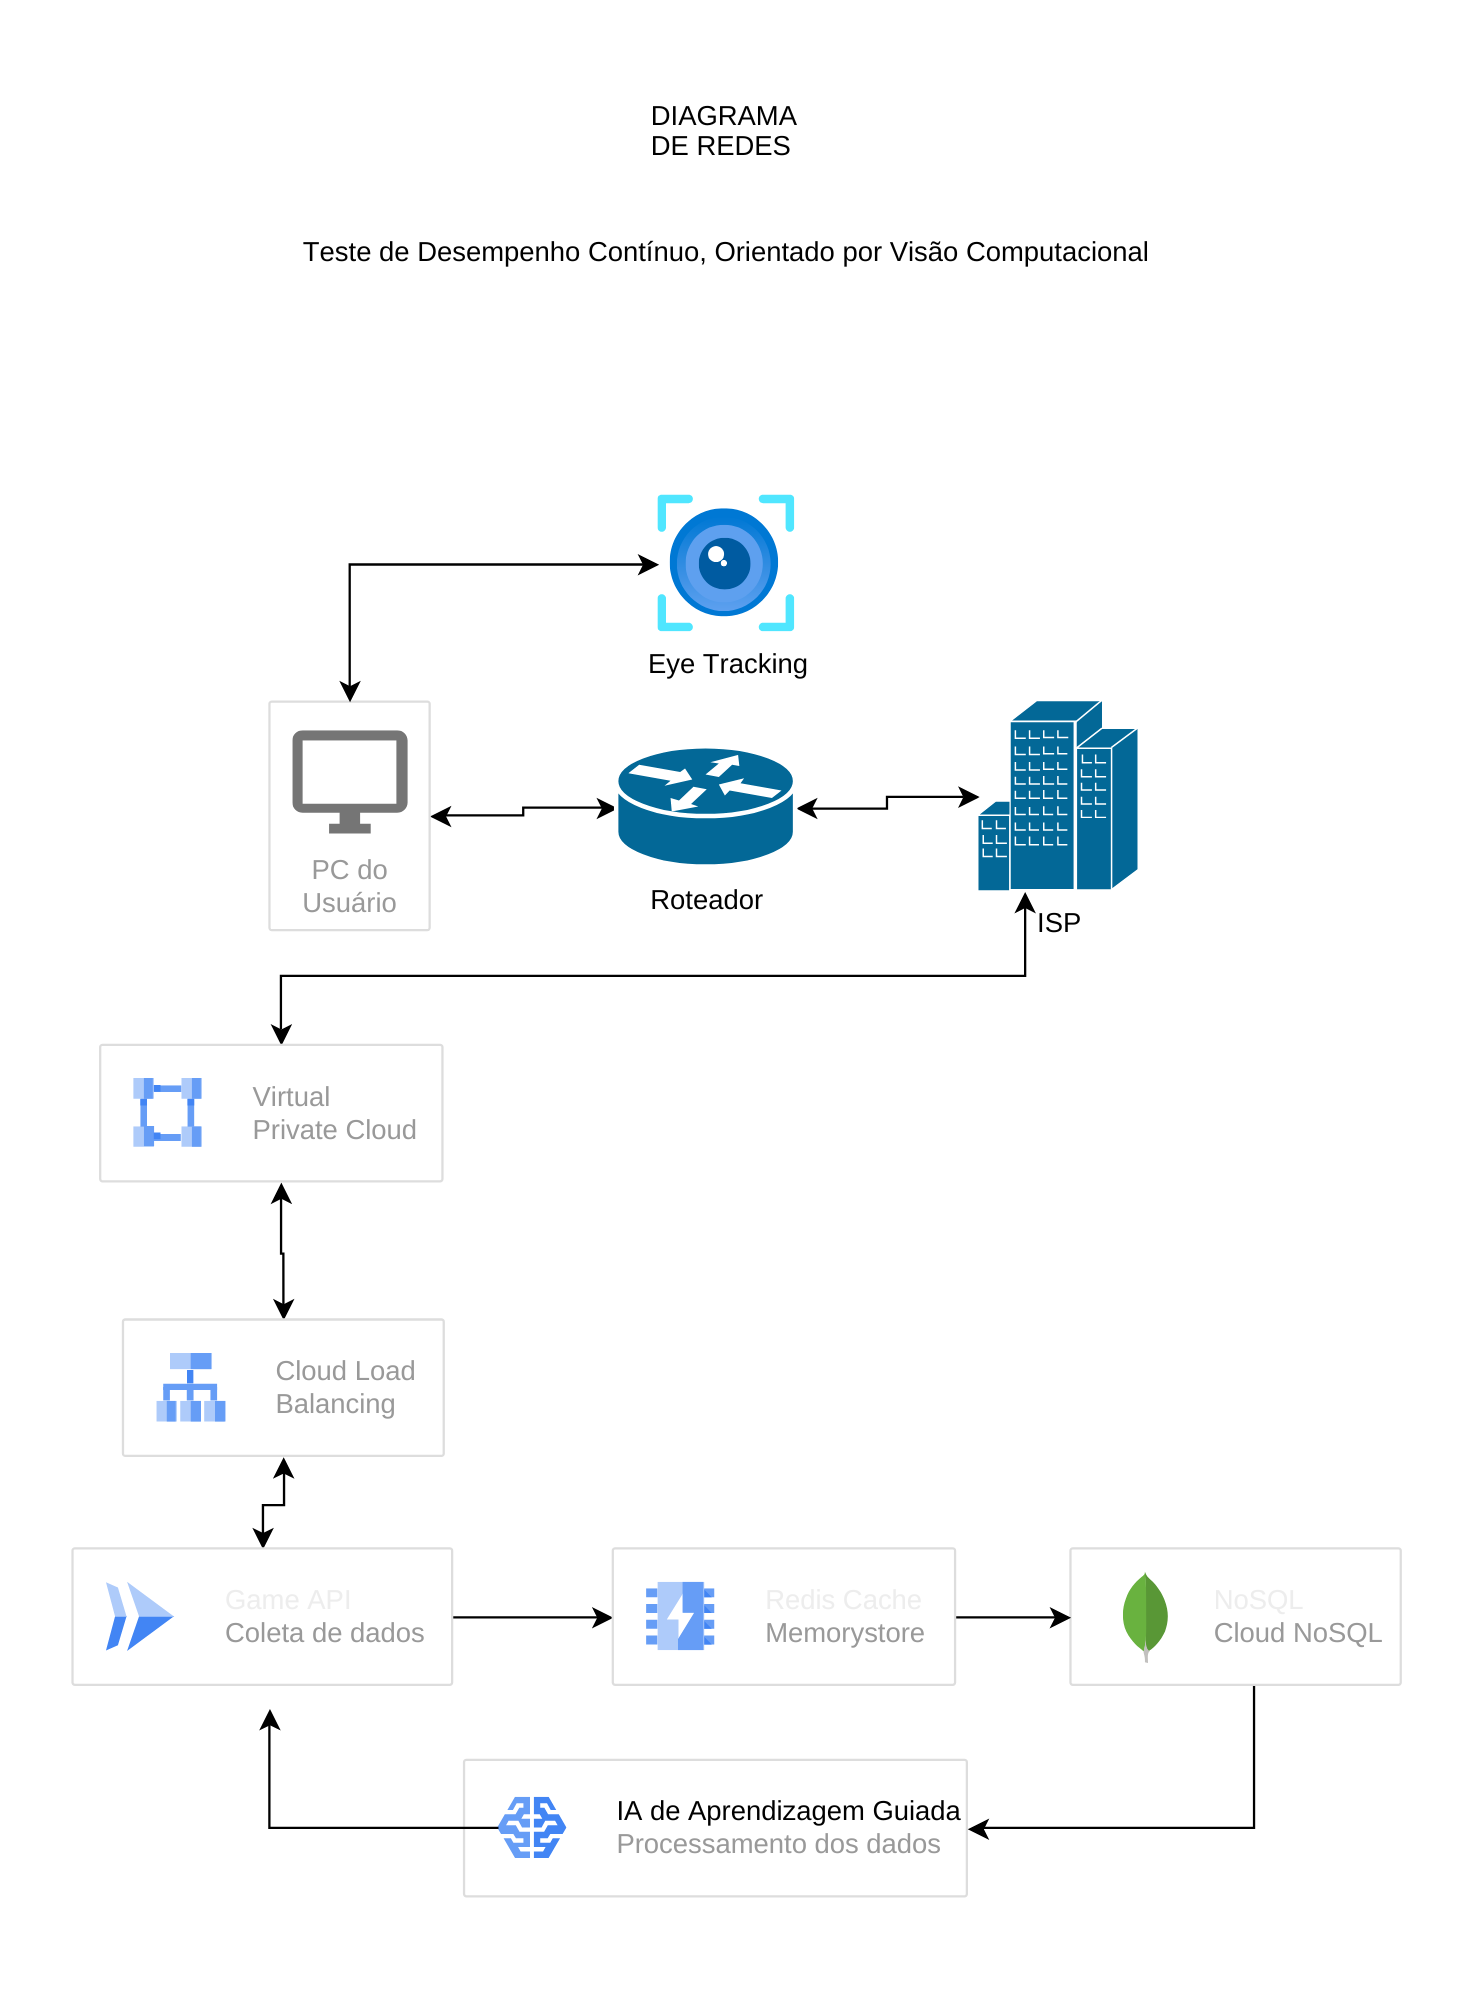
\includegraphics[width=\textwidth]{imgs/diagrama-redes.png}
\caption{Diagrama de Redes do Sistema}
\label{fig:network-diagram}
\end{figure}

\subsection{Pipeline CI/CD}

O pipeline de integração e entrega contínua do projeto é definido em \texttt{cloudbuild.yaml}. O fluxo automatiza a construção das imagens Docker, o envio para o Artifact Registry e o deploy dos serviços frontend e backend no Cloud Run. O backend é publicado com parâmetros de execução específicos, como \texttt{NODE	extunderscore ENV=production}, \texttt{PORT=4000}, \texttt{min-instances=3} e \texttt{max-instances=20}. O frontend é publicado separadamente, com \texttt{PORT=3000}, escalabilidade menor e variável \texttt{NEXT	extunderscore PUBLIC	extunderscore API	extunderscore URL} injetada via Secret Manager.

\begin{figure}[H]
\centering
\begin{tikzpicture}[
    node distance=1.5cm,
    every node/.style={rectangle, draw, rounded corners,
                       fill=secondarycolor!20,
                       text width=2cm,
                       align=center,
                       font=\small,
                       minimum height=1cm}
]
\node (code) {Code};
\node (test) [right of=code, xshift=1cm] {Test (GitHub Actions)};
\node (build) [right of=test, xshift=1cm] {Build (Cloud Build)};
\node (deploy) [right of=build, xshift=1cm] {Deploy (Cloud Run)};
\node (monitor) [right of=deploy, xshift=1cm] {Monitor};

\draw[->, thick] (code) -- (test);
\draw[->, thick] (test) -- (build);
\draw[->, thick] (build) -- (deploy);
\draw[->, thick] (deploy) -- (monitor);
\draw[->, thick, dashed] (monitor) to[bend right=45] (code);
\end{tikzpicture}
\caption{Pipeline CI/CD do FocusQuest}
\label{fig:cicd-focusquest}
\end{figure}

\subsection{Configuração CI/CD}

\begin{verbatim}
steps:

# Backend - Build Docker image

- name: 'gcr.io/cloud-builders/docker'
id: 'backend-build'
args:
- 'build'
- '-t'
- 'us-central1-docker.pkg.dev/$PROJECT_ID/focusquest/backend:$SHORT_SHA'
- '-t'
- 'us-central1-docker.pkg.dev/$PROJECT_ID/focusquest/backend:latest'
- '-f'
- 'backend-rastreamento-ocular/Dockerfile'
- 'backend-rastreamento-ocular/'
waitFor: ['-']



# Backend - Push to Artifact Registry

- name: 'gcr.io/cloud-builders/docker'
id: 'backend-push'
args:
- 'push'
- 'us-central1-docker.pkg.dev/$PROJECT_ID/focusquest/backend:$SHORT_SHA'
waitFor: ['backend-build']



# Frontend - Build Docker image

- name: 'gcr.io/cloud-builders/docker'
id: 'frontend-build'
args:
- 'build'
- '-t'
- 'us-central1-docker.pkg.dev/$PROJECT_ID/focusquest/frontend:$SHORT_SHA'
- '-t'
- 'us-central1-docker.pkg.dev/$PROJECT_ID/focusquest/frontend:latest'
- '-f'
- 'FocusQuest-web/Dockerfile'
- 'FocusQuest-web/'
waitFor: ['-']



# Frontend - Push to Artifact Registry

- name: 'gcr.io/cloud-builders/docker'
id: 'frontend-push'
args:
- 'push'
- 'us-central1-docker.pkg.dev/$PROJECT_ID/focusquest/frontend:$SHORT_SHA'
waitFor: ['frontend-build']



# Backend - Deploy to Cloud Run

- name: 'gcr.io/cloud-builders/run'
id: 'backend-deploy'
args:
- 'deploy'
- 'focusquest-backend'
- '--image'
- 'us-central1-docker.pkg.dev/$PROJECT_ID/focusquest/backend:$SHORT_SHA'
- '--region'
- 'us-central1'
- '--platform'
- 'managed'
- '--memory'
- '1Gi'
- '--cpu'
- '2'
- '--vpc-connector'
- 'focusquest-connector'
- '--vpc-egress'
- 'private-ranges-only'
- '--timeout'
- '3600'
- '--min-instances'
- '3'
- '--max-instances'
- '20'
- '--allow-unauthenticated'
- '--set-env-vars'
- 'NODE_ENV=production,PORT=4000,REDIS_PORT=6379,JWT_EXPIRACAO=1d'
- '--update-secrets'
- 'MONGO_URI=MONGO_URI:latest,REDIS_HOSTNAME=REDIS_HOSTNAME:latest,JWT_SECRET=JWT_SECRET:latest,FRONTEND_ORIGINS=FRONTEND_ORIGINS:latest'
env:
- 'CLOUDSDK_RUN_REGION=us-central1'
waitFor: ['backend-push']



# Frontend - Deploy to Cloud Run

- name: 'gcr.io/cloud-builders/run'
id: 'frontend-deploy'
args:
- 'deploy'
- 'focusquest-frontend'
- '--image'
- 'us-central1-docker.pkg.dev/$PROJECT_ID/focusquest/frontend:$SHORT_SHA'
- '--region'
- 'us-central1'
- '--platform'
- 'managed'
- '--memory'
- '512Mi'
- '--cpu'
- '1'
- '--timeout'
- '3600'
- '--min-instances'
- '2'
- '--max-instances'
- '10'
- '--allow-unauthenticated'
- '--set-env-vars'
- 'NODE_ENV=production,PORT=3000'
- '--update-secrets'
- 'NEXT_PUBLIC_API_URL=API_URL:latest'
env:
- 'CLOUDSDK_RUN_REGION=us-central1'
waitFor: ['frontend-push']



# Configuração de imagens

images:

- 'us-central1-docker.pkg.dev/$PROJECT_ID/focusquest/backend:$SHORT_SHA'
- 'us-central1-docker.pkg.dev/$PROJECT_ID/focusquest/backend:latest'
- 'us-central1-docker.pkg.dev/$PROJECT_ID/focusquest/frontend:$SHORT_SHA'
- 'us-central1-docker.pkg.dev/$PROJECT_ID/focusquest/frontend:latest'

# Opções de build

options:
machineType: 'N1_HIGHCPU_8'
logging: CLOUD_LOGGING_ONLY
substitution_option: 'ALLOW_LOOSE'

# Timeout total

timeout: '3600s'

# Substituições customizadas

substitutions:
_REGION: 'us-central1'
_SERVICE_ACCOUNT: 'focusquest-deploy'
\end{verbatim}

\subsection{Infraestrutura como Código}

\begin{table}[H]
\centering
\caption{Ferramentas DevOps Utilizadas}
\label{tab:devops-tools}
\begin{tabular}{|l|l|p{6cm}|}
\hline
\textbf{Categoria} & \textbf{Ferramenta} & \textbf{Finalidade} \\
\hline
Controle de Versão & Git + GitHub & Versionamento do código-fonte e acionamento de pipelines \\
Execução de aplicações & Cloud Run & Hospedagem serverless de frontend e backend com auto scaling e HTTPS \\
Containerização & Docker & Empacotamento do frontend e backend \\
Balanceamento de carga & Cloud Load Balancer & Distribuição de tráfego, TLS/SSL e suporte a WebSocket \\
CDN & Cloud CDN & Cache global para assets estáticos (imagens, CSS, JS)  \\
Cache / Mensageria & Memorystore for Redis & Cache em tempo real e comunicação distribuída entre instâncias \\
Banco de dados & MongoDB Atlas & Persistência principal dos dados da aplicação \\
Armazenamento & Cloud Storage & Armazenamento de backups e logs com versionamento e recuperação \\
Gerenciamento de segredos & Secret Manager & Armazenamento seguro de credenciais e variáveis sensíveis \\
Monitoramento & Cloud Monitoring e Logging  & Observabilidade de CPU, memória, latência e centralização de logs \\
CI/CD & Cloud Build & Automação de build, push de imagens e deploy contínuo \\
Rede & VPC Network & Isolamento de rede e comunicação privada entre serviços \\
Provisionamento & Scripts shell & Setup da rede, Redis, Artifact Registry e deploy \\
\hline
\end{tabular}
\end{table}

\subsection{Infraestrutura do Sistema}

Esta seção documenta como o sistema FocusQuest funciona em diferentes ambientes e plataformas.

\subsubsection{Arquitetura de Rede}

\begin{table}[H]
\centering
\caption{Componentes de Infraestrutura}
\label{tab:infrastructure}
\begin{tabular}{|l|p{10cm}|}
\hline
\textbf{Componente} & \textbf{Descrição} \\
\hline
\textbf{Ambiente Local (Desenvolvimento)} & 
\begin{itemize}[leftmargin=*, nosep]
    \item Backend Node.js e frontend Next.js executados localmente para desenvolvimento
    \item Banco MongoDB e cache Redis via Docker Compose para testes e validações
    \item Configuração por variáveis de ambiente para simular integrações de produção
    \item Suporte a testes manuais e automatizados antes do deploy
\end{itemize} \\
\hline
\textbf{Cloud (Produção/Staging)} & 
\begin{itemize}[leftmargin=*, nosep]
    \item Serviços frontend e backend implantados em Cloud Run
    \item Build, push de imagens e deploy automatizados com Cloud Build
    \item Artifact Registry para versionamento e armazenamento das imagens Docker
    \item Auto-scaling configurado por serviço (frontend e backend com limites próprios)
    \item Integração com VPC Connector para acesso privado a serviços internos
\end{itemize} \\
\hline
\textbf{Dados e Mensageria} & 
\begin{itemize}[leftmargin=*, nosep]
    \item MongoDB para persistência de usuários, pacientes, experimentos e resultados
    \item Redis (Memorystore) para cache, sessão e sincronização em tempo real
    \item Suporte a comunicação distribuída do Socket.io em múltiplas instâncias
    \item Estratégia de retenção e backup para continuidade operacional
\end{itemize} \\
\hline
\textbf{Cliente e Tempo Real} & 
\begin{itemize}[leftmargin=*, nosep]
    \item Aplicação web com rastreamento ocular híbrido (processamento local + backend)
    \item Comunicação REST para operações de negócio e WebSocket para eventos em tempo real
    \item Encaminhamento de rotas de API do frontend para backend por configuração de ambiente
    \item Atualização de análises em tempo real para fases experimentais
\end{itemize} \\
\hline
\end{tabular}
\end{table}

\subsubsection{Diagrama de Infraestrutura}

Para ilustrar como os componentes se conectam:

\begin{figure}[H]
\centering
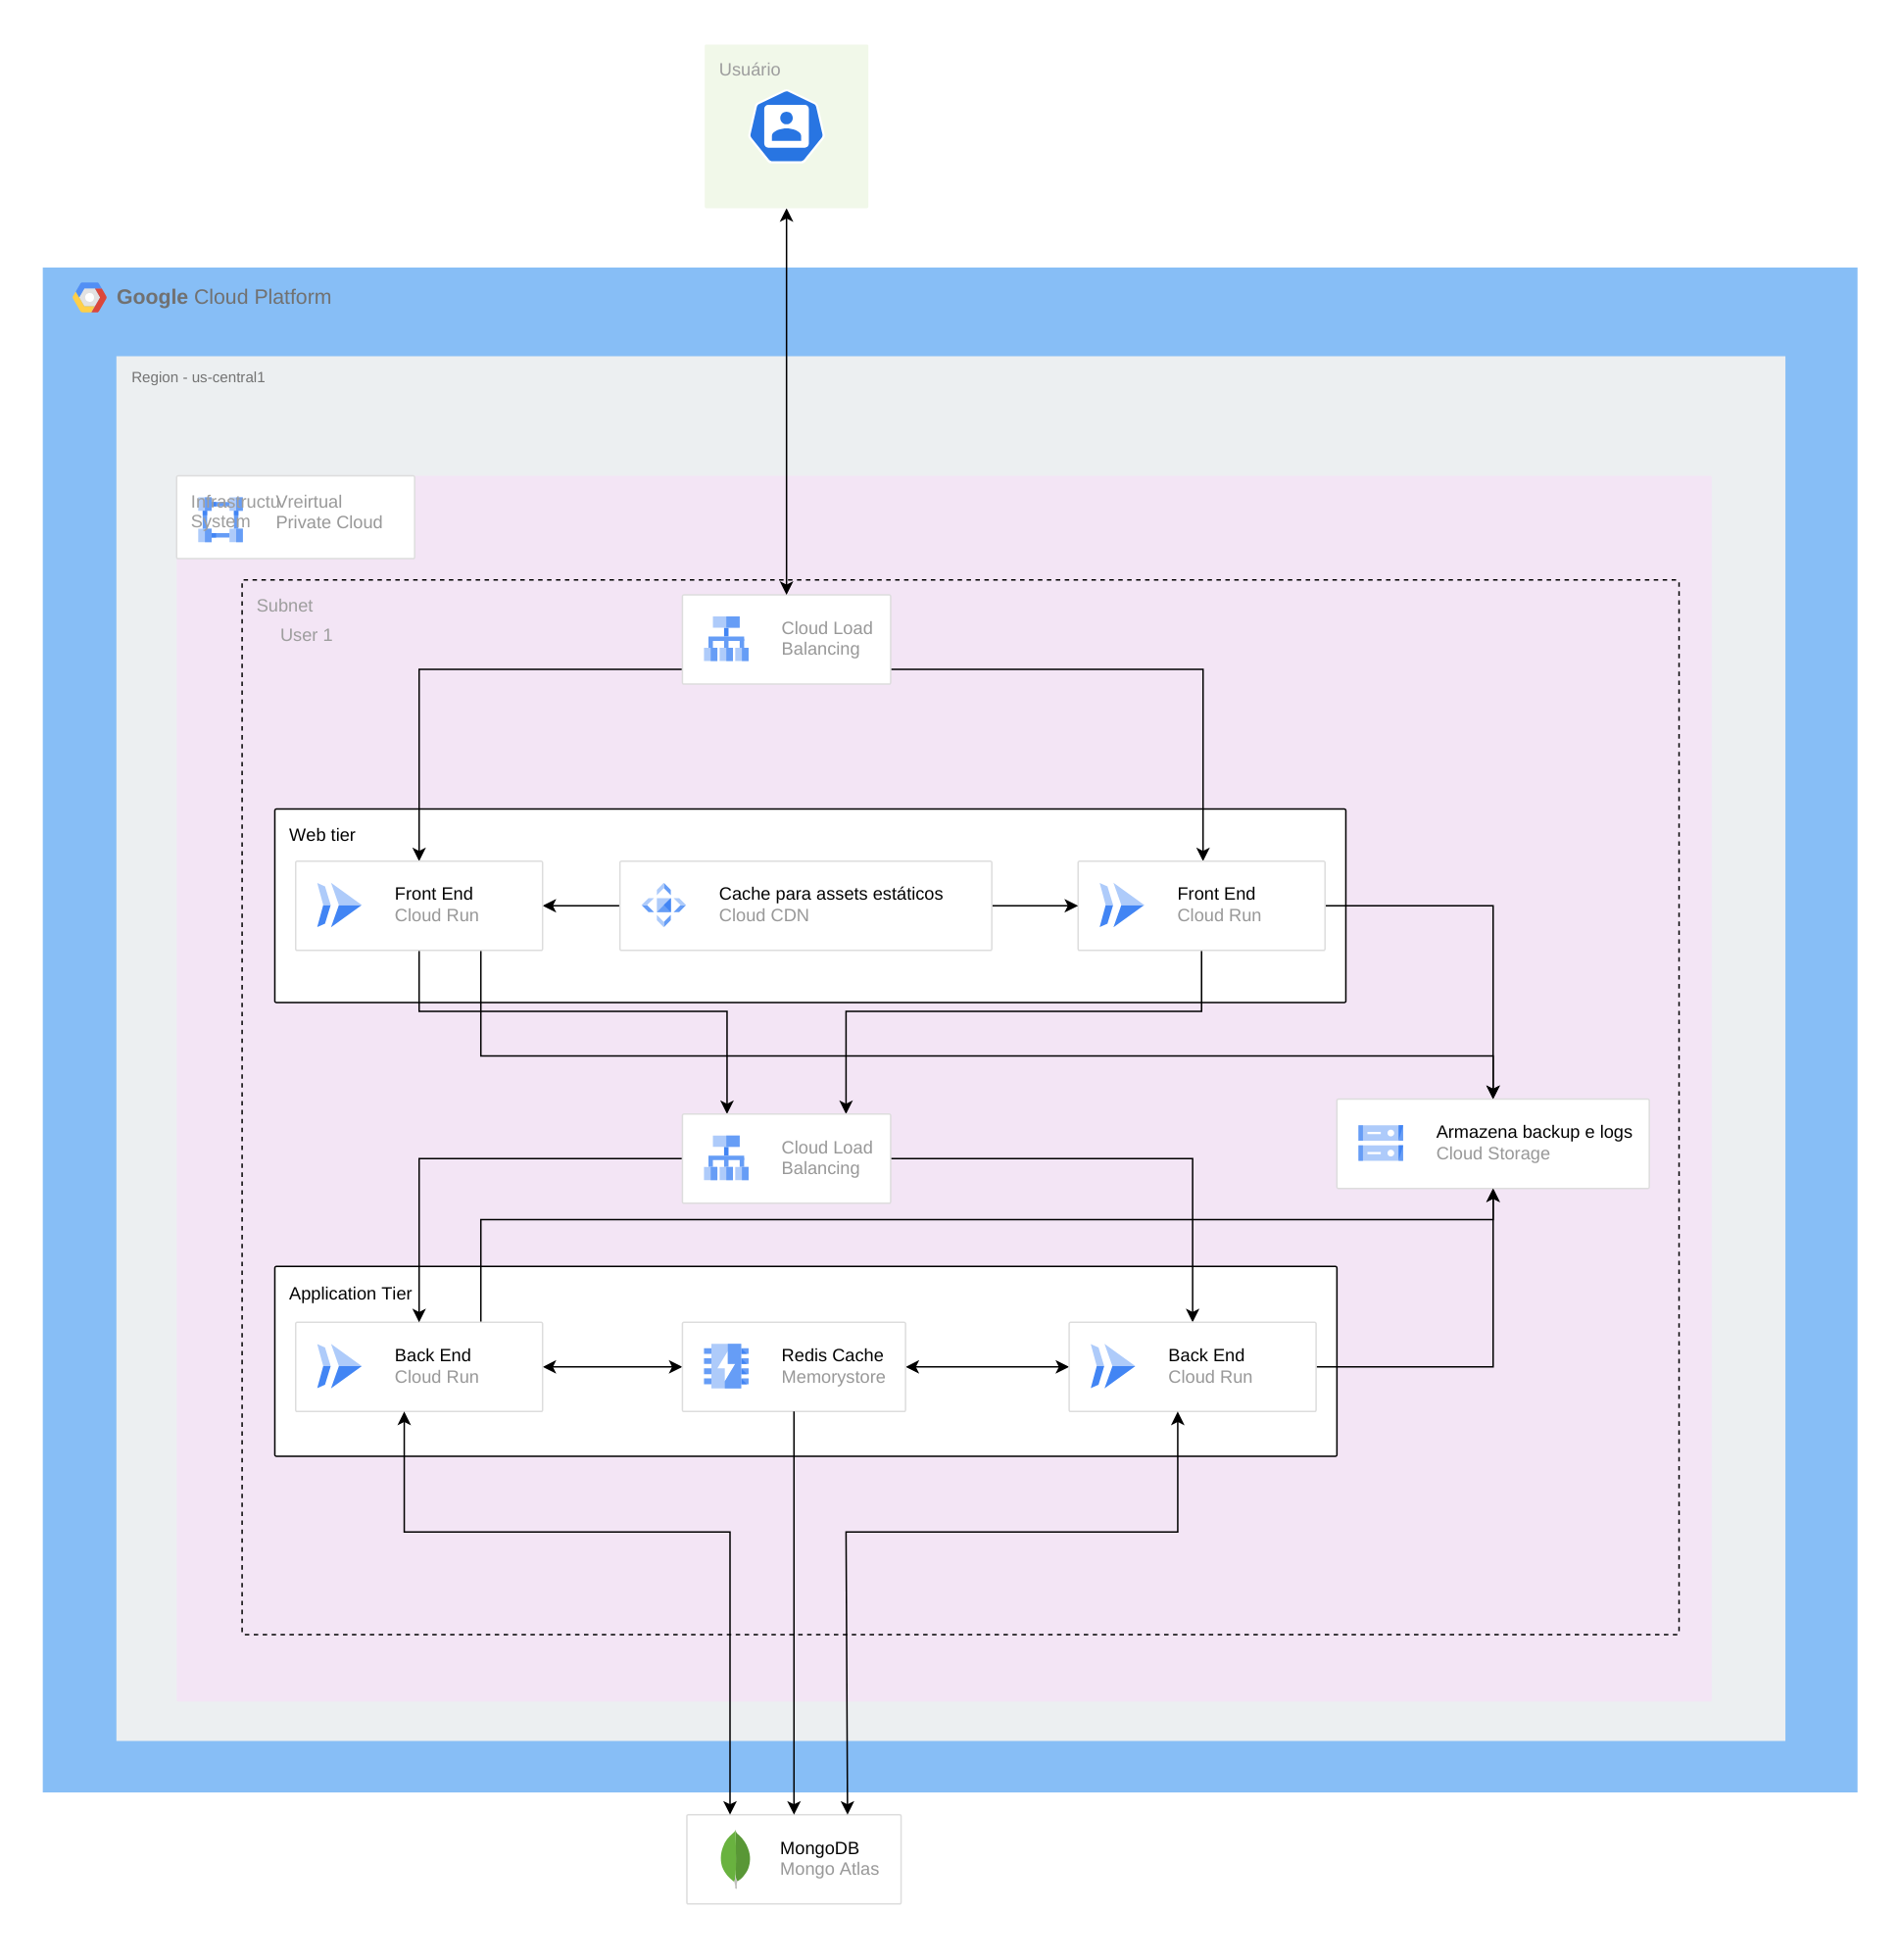
\includegraphics[width=\textwidth]{imgs/diagrama-infra.png}
\caption{Diagrama de Infraestrutura do Sistema}
\label{fig:infrastructure-diagram}
\end{figure}

\textbf{Exemplo de descrição:}

\begin{itemize}
    \item \textbf{Usuários Web:} Acessam via navegador através de HTTPS
    \item \textbf{Usuários Mobile:} Conectam-se via API REST com autenticação
    \item \textbf{Banco de Dados:} PostgreSQL em cluster para alta disponibilidade
    \item \textbf{Storage:} Amazon S3 para arquivos e imagens
    \item \textbf{Cache:} Redis para otimização de performance
    \item \textbf{Fila de Mensagens:} RabbitMQ para processamento assíncrono
\end{itemize}

\subsection{Arquitetura de Deploy}

\begin{figure}[H]
\centering
\begin{tikzpicture}[
    node distance=2.5cm,
    component/.style={rectangle, draw, rounded corners, 
                      fill=secondarycolor!20, 
                      text width=2.5cm, 
                      align=center,
                      minimum height=1.2cm}
]
\node[component] (lb) {Load Balancer};
\node[component, below left of=lb] (app1) {Frontend Cloud Run};
\node[component, below right of=lb] (app2) {Backend Cloud Run};
\node[component, below left of=app2] (db) {MongoDB};
\node[component, below right of=app2] (cache) {Redis Cache};

\draw[<->, thick] (lb) -- (app1);
\draw[<->, thick] (lb) -- (app2);
\draw[<->, thick] (app1) -- (app2);
\draw[<->, thick] (app2) -- (db);
\draw[<->, thick] (app2) -- (cache);
\end{tikzpicture}
\caption{Arquitetura de Deployment}
\label{fig:deployment}
\end{figure}

\subsection{Métricas e SLA}

Para o ambiente do FocusQuest, as métricas de operação podem ser definidas com base na arquitetura em Cloud Run, com backend Node.js, frontend Next.js, Redis e MongoDB.

\begin{itemize}
    \item \textbf{Disponibilidade:} 99.5\% a 99.9\%
    \item \textbf{Tempo de Resposta Médio:} < 300ms para rotas REST simples
    \item \textbf{Tempo de Resposta P95:} < 800ms
    \item \textbf{Taxa de Erro:} < 1\%
    \item \textbf{Throughput:} 300 a 800 requisições/segundo em carga normal
    \item \textbf{Latência WebSocket:} < 100ms para eventos em tempo real
    \item \textbf{Deploy Frequency:} diário ou sob demanda
    \item \textbf{Lead Time:} < 2 horas para alterações pequenas
    \item \textbf{MTTR:} < 30 minutos
    \item \textbf{Escalabilidade Backend:} 3 a 20 instâncias
    \item \textbf{Escalabilidade Frontend:} 2 a 10 instâncias
\end{itemize}

\newpage
\section*{Conclusão}

Este documento apresenta os principais artefatos necessários para a documentação completa de um projeto de software. Cada seção fornece exemplos práticos de como inserir e formatar os diferentes tipos de artefatos utilizando \LaTeX.

Os artefatos documentados incluem:
\begin{itemize}
    \item \textbf{CANVAS:} Modelo de negócio e estratégia
    \item \textbf{SWOT:} Análise estratégica de forças, fraquezas, oportunidades e ameaças
    \item \textbf{UX/UI:} Design de interface e experiência do usuário
    \item \textbf{Website:} Estrutura e especificações técnicas web
    \item \textbf{Diagramas UML:} Modelagem visual do sistema
    \item \textbf{Banco de Dados:} Modelagem e estruturação de dados
    \item \textbf{DevOps:} Infraestrutura, automação e práticas de entrega contínua
\end{itemize}

\newpage
\addcontentsline{toc}{section}{Referências}
\bibliographystyle{plainnat}
\bibliography{referencias}

\end{document}
